\section{Results}
Here, we set the parameters as default values and observe its performance. Our default parameters are set based on three simple rule. Firstly, because of the different numbers of hydrogen bonds between A/T and C/G, the energy decrease due to A/T binding are 1.5 times to C/G binding. So the parameter\#1 is 1.5 times parameter\#2. Secondly, it's universally known that big compounds with small distance will have a high energy because of repulsion. The mismatching combination between two nucleotides can be classified into three parts--large, medium and small, and we should set other parameters in the same order of values. Thirdly, we use the parameters from \cite{klein2018hybridization} as reference. In total, we set the parameters default values as [0.06,0.09,0.3,0.6,0.03].

 As the following figure shows, the energy always decreases or has some turning point because of mismatch and is always negative. The yellow line represents complete match. The blue line and the red line are two examples of mismatches at different positions. For example, the red line has a peak due to a mismatch, and in our model, we find that it doesn't make the energy positive. It means that in this reaction process there is some force like "momentum" pushing it to proceed and cross the energy peak. For a off-target examination to every location of all the DNA in a system (a genome), there will also be positive energy result, which is obviously not a feasible solution (will not lead to off-target). This kind of results is omitted in the plot.
\begin{figure}[H]
\centering
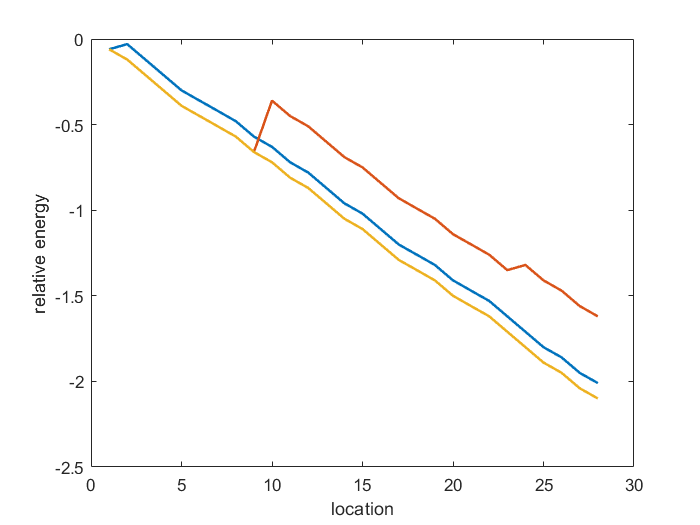
\includegraphics[width=0.7\linewidth]{energy_change}
\caption{Energy change of sgRNA candidates binding to DNA}
\label{fig:energychange}
\end{figure}

\begin{figure}[H]
\centering
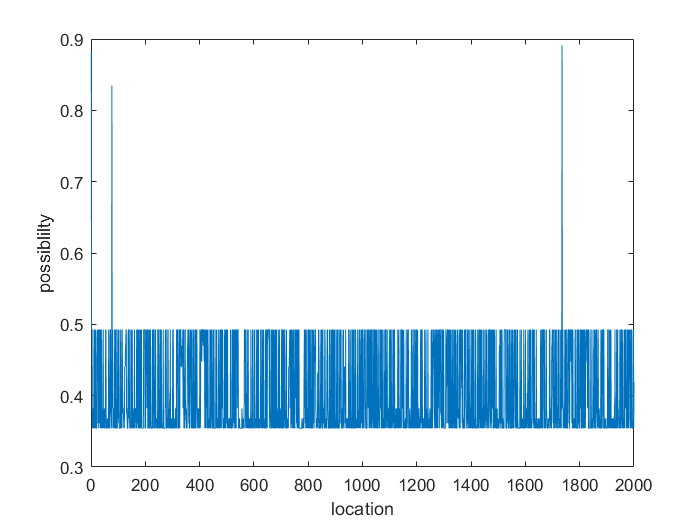
\includegraphics[width=0.7\linewidth]{fig1}
\caption{The possibility of sgRNA candidates binding to DNA's different locations}
\label{}
\end{figure}

After testing our code's running time, we find its rate can reach approximately $2\times10^8\;base/h$ (under parallel computing in 4 cores).

Besides the default parameters, we hope our model can hit more true data. So after we get the experiment data, we can use the parameter optimization method mentioned before to get more precise parameters. 
